\newtheorem{DEF}{Definition}

%=====================================================================================
\chapter{Introduction}

In these days, Continuous Integration (CI) is more often used in larger projects, where multiple developers are working on one and the same software product. This process ensures fast software development, called eXtreme Programming (XP), known as agile software development methodology. The methodology is mainly used to accelerate the development, nevertheless, development of software may be disrupted in various other ways. Nowadays, although this type of software development has many disadvantages, it is still much more often used on larger projects. The progress of the development may not be reached with a continuous integration which guarantees less disorder and failures. You may also know that the continuous integration is a part of the following open-source projects e.g. Facebook, Twitter, Mozilla. These projects use one of many famous continuous integration service Travis CI. Excluding Travis CI, there are plenty of other continuous integration services you may heard about, such as Jenkins, TeamCity, CircleCI, GitLab CI, Codeship and so on.\\

The software development process requires many code checking tools after every single code change in the source code. For as much as with every single change of code, there is a possibility to add, fix, derange or deteriorate any parts of the software product. These tools provide an automated code review and they afford a quick feedback by which they try to prevent these code impairments. Feedback about his adjustment is sent to the developer, who has made the change in the code. The automated process which provides the code review does not bother with executing a huge amount of tests. Above mentioned process is conducted via continuous integration server, which compiles the code, runs scripts and tests. The results are aggregated and the feedback is given to the developer who has made this code change. Continuous integration server is invoked every single time after any change is fetched in the source code and he had to execute the stated acts which are predefined. In next chapters we describe in details how does this workflow work and what steps are required to run.\\

The essence of this work is about the basics of continuous integration and its fundamentals. This thesis attempts to explain how the fundamentals of continuous integration and automated code review work. It describes how it is integrated to the software development, and how it works on an extensive project nowadays. Examples will be based on open-source project e.g. ManageIQ, which is a cloud manager founded by RedHat. The development process of the ManageIQ rests in agility and stability of the progress. These main factors of the development process could not be reached without a quick feedback to the developers working on project about their changes, that are submitted to the software product.

%=====================================================================================
\chapter{Continuous Integration \& Automated Code Review}

Despite the fact that continuous integration and automated code review are used in a lot of projects, it is still an unknown part of software development. There are only a few researches describing this part of development how is it deployed, managed and used. Development analysts are not giving an adequate attention to this part of software development. They are usually describing it as a common part of development in a software development process. This part is concerning to extreme programming due to fast code change deployment. This development technique is very adaptive and still more and more open source projects are using it. There are many of developers relying to this type of software development which helps them rapidly. This chapter will give you a detailed point of view above the modern in-use software development methodology which is still in evolution.

\section{Continuous Integration}
Continuous integration has a key role in the software development process consisting of a few certain unavoidable steps which will be described later in next subsections. Everything begins at the moment, when one developer who has made changes in a source code of the software product is trying to commit them into the software product. The process of continuous integration has begun at this point and lasts until feedback is sent back to the developer. These stages of continuous integrations are proceed every time after the CI server has detected a change in a version control repository. This automation has a lot of benefits which are necessary to keep the software product without any kind of defects. Many of them are detected in time and reported back to the developer as a corrupted source code. Not a few developers may think that the continuous integration is only about compiling a source code and launching tests. In the next subsections, we will present the steps of the continuous integration and describe these individual phases in detail.\\

\begin{figure}[H]
	\centering
	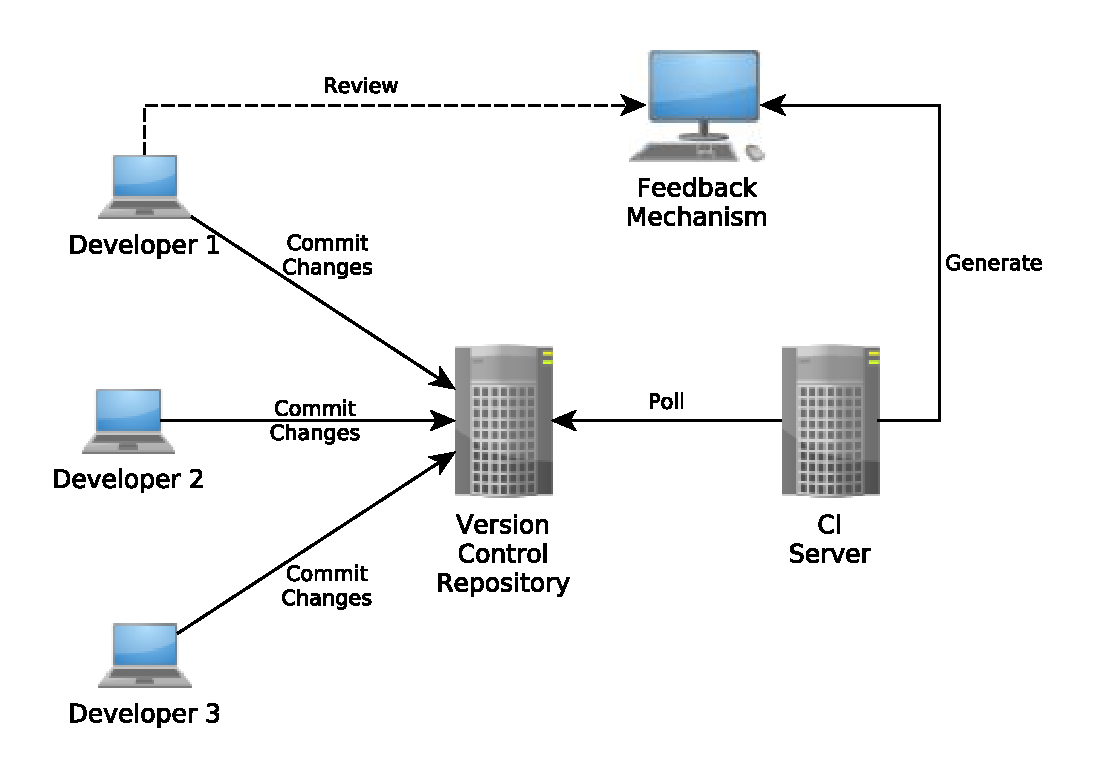
\includegraphics[scale=0.6]{yEd/components_of_CI_system.eps}
	\caption{Components of continuous integration system\cite{CI}}
	\label{fig:cocis}
\end{figure}

\subsection{Demands of continuous integration}
The minimal requirements for good software development of a project where multiple developers are working on a same project are a version control repository and a continuous integration server. The version control system guarantees a software configuration management which is required for the continuous integration. The meaning of the version control system is very important. You cannot manage changes that developers had made in the source code without a version control system. The version control system has a very positive impact on the developing project. The system offers a history of changes which may be highly useful if a rollback is desired. Besides the history of changes, this system may save more other information about the source code, e.g. who did the change, when was the change created, etc. In addition, the version control system is represents a primary source for the project source codes. This type of project setup is much more often used these days rather than in the past. Nearly every project has its own version control system which is provided by a repository hosting service.\\

A continuous integration server has a huge advantage. This is a reason why it is highly recommended. It depends on the developer, how does he deploy the continuous integration server. With the continuous integration server, he does not have to bother with such many scripts for the automation. Nevertheless, as he decides how the continuous integration server will be established, the system must contain these features. To facilitate the process of continuous integration, the system must support services as polling version control system, retention of build history, launching predefined steps such as scripts and tests. Furthermore, the system should offer an opportunity to send a feedback back to the developers. This server executes a series of actions or steps taken in order to achieve a particular end of continuous integration. The next subsection will determine and state these fundamental steps of the continuous integration scenario, describe and illustrate them in detail.

\subsection{Stages of continuous integration}

The stages of continuous integration insure code inspection and code integration. Before we begin, we need to clarify certain concepts which will be used later. To understand these steps, we need to understand what is the difference between \textbf{a build}, \textbf{a private build} and \textbf{an integration build}.

\begin{DEF}
A build may refer to a set of activities performed to generate, test, inspect, and deploy software\cite{CI}.
\end{DEF}

\begin{DEF}
A private build define a process in which a software developer runs the build on his local machine to ensure that the changes he made work, before he commits them into a version control repository.
\end{DEF}

\begin{DEF}
An integration build is the act of combining software components (programs and files) into a software system\cite{CI}.
\end{DEF}

Now as we know what are these concepts we will illustrate the basic acts of continuous integration. To describe it properly, imagine that we have a group of developers working on the same project using a version control system where is the source code of the software product held, and they are using a continuous integration service. The stages of continuous integration are the following:

\begin{enumerate}
	\item \textbf{The change}\\
		  One developer who wish like to make a change, adjustment, improvement or a new feature in the software product, has to clone the remote version control repository to his local computer to download the source code of the software product. At this point he has a local version control repository in which he will do the changes he would like to. After a made change, the change is only in local repository and the developer would like to commit them into remote repository. Before publishing the changes he has to run a private build. The developer has to publish the changes he made, which is a request for an approval of a change ready to merge into a specific branch on remote repository. These not merged changes are published on remote version control repository.\\
		  By committing changes to the version control repository invokes a continuous integration server. The continuous integration server is polling the version control repository in a periodic intervals and when a changes is detected than a reaction will occur.
	\item \textbf{The reaction}\\
		  When a change is detected it invokes a continuous integration server to execute a few tasks. Tasks are predefined in a build script which has to integrate the change with the rest of the source code of the software product. The script provide source code compilation, database integration, testing, code inspection. The execution of the script is referred to as an integration build.\\
		  This stage of continuous integration is known for code verification, it finds defects or errors made by developer which occur e.g. compilation fail, tests failures etc. The faultiness is reveal by tests which should have high code coverage. Failures of this stage can be reduced by launching a private build which may be less complex compared to launching the build script. Passing this stage depends on success of build script which must be success on 100\%.
	\item \textbf{The feedback}\\
		  Continuous integration server generates a feedback which is assigned to this change and it might be sent to the author of the change. There is a log information generated every time by passing stage before and it is held and assigned to the change. Feedback is given to the developer in a certain predefined form, e.g. email with failures only. The log file is saved on the continuous integration server where is a overview about the builds and their stats.
	\item \textbf{The waiting}\\
		  This stage is the end of the process, it stands for continuous polling of  the version control repository waiting for a new change in it. Detecting a change will cause launching the stages from the beginning.
\end{enumerate}



\section{Automated Code Review}
Abcd.

%=====================================================================================
\chapter{Continuous Integration in open source projects}
Asdf.

\section{Open source}
Asdf.

\section{Github}
Asdf.

\section{TravisCI}
Asdf.

%=====================================================================================
\chapter{Conclusion}
Asdf.

